\documentclass[12pt,a4paper]{report}

\usepackage[margin=2.0cm,headheight=14pt]{geometry}
\usepackage[T1]{fontenc}
\usepackage[utf8]{inputenc}
\usepackage[english]{babel}
\usepackage{lmodern}
\usepackage{microtype}
\usepackage{graphicx}
\usepackage{booktabs}
\usepackage{longtable}
\usepackage{array}
\usepackage{tabularx}
\usepackage{multirow}
\usepackage{xcolor}
\usepackage{colortbl}
\usepackage{tikz}
\usepackage{tcolorbox}
\tcbuselibrary{breakable,skins}
\usepackage{hyperref}
\usepackage{enumitem}
\usepackage{amsmath}
\usepackage{caption}
\usepackage{fancyhdr}
\usepackage{titlesec}
\usepackage{setspace}
\usepackage[backend=biber,style=ieee,sorting=none]{biblatex}

\addbibresource{references.bib}

% aivancity palette
\definecolor{aivanavy}{HTML}{1D2A4D}
\definecolor{aivagold}{HTML}{C5A045}
\definecolor{aivagray}{HTML}{F2F4F7}
\definecolor{aivatext}{HTML}{4A4A4A}

\hypersetup{
  colorlinks=true,
  linkcolor=aivanavy,
  citecolor=aivanavy,
  urlcolor=aivanavy,
  pdftitle={AI CLINIC REPORT},
  pdfauthor={Remi Uttejitha ALLAM, Baptiste Langlois, Tong Li, Darryl Towa}
}

\titleformat{\chapter}[hang]
  {\normalfont\Large\bfseries\color{aivanavy}}
  {\thechapter.}{0.6em}{}
\titleformat{\section}{\normalfont\large\bfseries\color{aivanavy}}{\thesection}{0.7em}{}
\titleformat{\subsection}{\normalfont\normalsize\bfseries\color{aivanavy}}{\thesubsection}{0.6em}{}
\titleformat{\subsubsection}{\normalfont\bfseries\color{aivanavy}}{\thesubsubsection}{0.5em}{}
\titlespacing*{\chapter}{0pt}{8pt}{6pt}
\titlespacing*{\section}{0pt}{8pt}{3pt}
\titlespacing*{\subsection}{0pt}{6pt}{2pt}
\titlespacing*{\subsubsection}{0pt}{4pt}{2pt}

\pagestyle{fancy}
\fancyhf{}
\fancyfoot[C]{\thepage}
\renewcommand{\headrulewidth}{0pt}

\setstretch{1.05}
\setlist[itemize]{topsep=2pt,itemsep=1pt,parsep=0pt,partopsep=0pt}
\setlist[enumerate]{topsep=2pt,itemsep=1pt,parsep=0pt,partopsep=0pt}

\setlength{\abovecaptionskip}{4pt}
\setlength{\belowcaptionskip}{2pt}
\setlength{\textfloatsep}{8pt plus 2pt minus 2pt}
\setlength{\floatsep}{6pt plus 2pt minus 2pt}
\setlength{\intextsep}{6pt plus 2pt minus 2pt}
\setlength{\parskip}{2pt}
\renewcommand{\baselinestretch}{1.05}

% ---------------------------------------------------------------------------
% Title-page fields
% ---------------------------------------------------------------------------
\newcommand{\ProjectTitle}{AI for Healthcare Compliance and Regulations Across Countries}
\newcommand{\ProjectSubtitle}{Interactive Dashboard and Comparative Regulatory Analysis}
\newcommand{\StudentNames}{Remi Uttejitha ALLAM, Baptiste Langlois, Tong Li, Darryl Towa}
\newcommand{\SupervisorName}{Dr.\ Anuradha Kar}
\newcommand{\HostOrganisation}{AI Clinic}
\newcommand{\AcademicYear}{2025--2026}
\newcommand{\SubmissionDate}{30 August 2026}

\begin{document}

% ===========================================================================
% 1. TITLE PAGE
% ===========================================================================
\begin{titlepage}
\hypersetup{pageanchor=false}
\thispagestyle{empty}
\centering

\vspace*{0.2cm}

\includegraphics[width=0.52\textwidth]{assets/aivancity_logo.png}

\vspace{0.7cm}

\noindent

\begin{tikzpicture}
  \fill[aivanavy] (0,0) rectangle (\textwidth,1.45cm);
  \node[anchor=west, inner sep=0pt] at (0.45cm,0.98cm)
    {\color{white}\bfseries\large Grande \'Ecole Program};
  \node[anchor=west, inner sep=0pt] at (0.45cm,0.42cm)
    {\color{aivagold}\itshape Specialization: Artificial Intelligence \& Data Science};
\end{tikzpicture}

\vspace{0.9cm}

\begin{flushleft}
{\color{aivagold}\rule{0.35cm}{1.4cm}}%
\hspace{0.35cm}%
\begin{minipage}[t]{0.88\textwidth}
  {\color{aivatext}\small\bfseries AI CLINIC\par}
  \vspace{0.25cm}
  {\color{aivanavy}\LARGE\bfseries \ProjectTitle\par}
  \vspace{0.25cm}
  {\color{aivagold}\large\itshape \ProjectSubtitle\par}
\end{minipage}
\end{flushleft}

\vspace{1.0cm}

\noindent
\begin{tcolorbox}[
  colback=aivagray,
  colframe=aivagray,
  boxrule=0pt,
  arc=2pt,
  left=14pt,
  right=14pt,
  top=12pt,
  bottom=12pt,
  width=\textwidth
]
\renewcommand{\arraystretch}{1.55}
{\color{aivatext}\normalsize
\begin{tabular}{@{}>{\bfseries}p{4.3cm} p{\dimexpr\linewidth-4.5cm\relax}@{}}
Names & Remi Uttejitha ALLAM \\
      & Baptiste Langlois \\
      & Tong Li \\
      & Darryl Towa \\
Supervisor & \SupervisorName \\
Academic year & \AcademicYear \\
Submission date & \SubmissionDate \\
\end{tabular}}
\end{tcolorbox}

\end{titlepage}

\hypersetup{pageanchor=true}
\pagenumbering{roman}

% ---------------------------------------------------------------------------
\chapter*{Acknowledgements}
\addcontentsline{toc}{chapter}{Acknowledgements}

We thank our supervisor, \SupervisorName, for guidance throughout this AI Clinic project. We also thank aivancity School of AI \& Data for Business \& Society for the academic setting in which this work was carried out. Primary regulatory texts, international guidance, and peer-reviewed literature cited in this report remain the property of their respective authors and institutions.

% ---------------------------------------------------------------------------
\chapter*{Abstract}
\addcontentsline{toc}{chapter}{Abstract}

Artificial intelligence (AI) is reshaping healthcare through diagnostic imaging, digital pathology, genomic interpretation, drug-discovery support, and clinical decision support. These capabilities create substantial regulatory complexity: software may qualify as Software as a Medical Device (SaMD), process sensitive health data under divergent privacy regimes, and require lifecycle governance when algorithms adapt over time.

This project delivers a research and engineering artefact comprising (1)~a structured literature review of AI healthcare compliance across 20 countries in six regions; (2)~a curated dataset scoring seven regulatory themes on a 1--10 scale; and (3)~an interactive dashboard for geospatial comparison, theme analysis, global trends, use-case readiness, and literature browsing.

Key findings include convergence toward risk-based SaMD classification and comprehensive data protection modelled on the GDPR, persistent disparities in enforcement capacity between advanced and emerging economies, and growing emphasis on post-market surveillance and liability for adaptive AI. The EU AI Act is a watershed in binding AI governance. Clinical adoption in radiology, pathology, genomics, and public-health surveillance amplifies the need for transparent validation, representative datasets, and Total Product Lifecycle oversight.

\textbf{Keywords:} AI healthcare regulation; SaMD; compliance dashboard; data privacy; clinical validation; EU AI Act; post-market surveillance.

\tableofcontents
\clearpage
\chapter*{List of Tables and Figures}
\addcontentsline{toc}{chapter}{List of Tables and Figures}
\vspace{-0.4em}
{\small
\section*{List of Tables}
\makeatletter
\@starttoc{lot}
\makeatother
\vspace{0.6em}
\section*{List of Figures}
\makeatletter
\@starttoc{lof}
\makeatother
}
\clearpage
\pagenumbering{arabic}

% ===========================================================================
\chapter{Introduction}
\label{ch:intro}
% ===========================================================================

\section{General context}

The integration of AI into healthcare is one of the most consequential technological shifts of the twenty-first century. AI-based SaMD now assists clinicians in radiology, pathology, ophthalmology, cardiology, and genomics, among other specialties \cite{topol2019,rajpurkar2022}. Major regulators have authorised hundreds of AI/ML-enabled devices, reflecting exponential growth in the field \cite{fda2021,wu2021}.

Unlike traditional medical devices, AI systems can be adaptive, opaque, and dependent on training data that may embed biases---raising regulatory questions that existing frameworks were not designed to address \cite{gerke2020,char2018}. Ensuring patient safety, data privacy, algorithmic fairness, and accountability therefore requires jurisdiction-specific compliance strategies and continuous monitoring after deployment.

\section{Problem statement}

Regulatory diversity across countries creates practical and scholarly difficulties for four groups of stakeholders:
\begin{itemize}
  \item \textbf{Developers} seeking international market access and harmonised evidence packages;
  \item \textbf{Researchers} studying comparative AI governance;
  \item \textbf{Policymakers} balancing innovation incentives with safety protections;
  \item \textbf{Clinicians and hospital administrators} evaluating whether AI tools meet local legal and ethical requirements.
\end{itemize}

Public information on AI healthcare regulation is abundant but fragmented: statutes, guidance, ethics principles, and device-authorisation lists sit in separate institutional silos. There is a need for a structured, comparative analysis that is both scholarly (literature synthesis, explicit scoring method) and usable (an interactive dashboard). This project addresses that gap by combining a coded 20-country dataset with a visual analytics interface.

\subsection{Project objectives}

The project aims to:
\begin{enumerate}
  \item Synthesise peer-reviewed and policy literature on AI healthcare regulation across 20 countries;
  \item Define seven thematic dimensions of compliance and score jurisdictional maturity on a 1--10 scale;
  \item Build a curated, machine-readable dataset with regional metadata and global trends;
  \item Implement an interactive dashboard for exploration, comparison, and literature browsing;
  \item Document methodology, architecture, and findings in this report.
\end{enumerate}

\subsection{Scope and limitations}

The analysis covers 20 countries across North America, Europe, East Asia, South/Southeast Asia, the Middle East, Africa, and Oceania. Theme scores are expert-curated syntheses informed by regulatory documents and literature---they are comparative indicators, not official government ratings. Use-case readiness scores in the dashboard are \emph{derived} from theme weights rather than separate regulatory datasets. This report is an academic and decision-support artefact, not legal advice.

\section{Literature review}
\label{sec:lit}

This section synthesises regulatory frameworks, privacy regimes, clinical-evidence expectations, ethics, surveillance, and liability for AI in healthcare, drawing on sources from 2018--2026.

\subsection{Regulatory frameworks for AI medical devices}

The IMDRF framework (2014) provides foundational categorisation for software that meets the definition of a medical device without being part of hardware \cite{imdrf2014}. Major jurisdictions have adopted or adapted it:
\begin{itemize}
  \item \textbf{United States:} the FDA regulates AI/ML SaMD via 510(k), De Novo, and PMA pathways, supplemented by the AI/ML SaMD Action Plan \cite{fda2021};
  \item \textbf{European Union:} the MDR classifies SaMD by intended purpose and risk; the EU AI Act adds high-risk AI obligations \cite{euaiact2024};
  \item \textbf{Japan:} the PMDA administers the DASH framework for SaMD \cite{pmda2020};
  \item \textbf{China:} the NMPA issued guiding principles for AI medical-device registration \cite{nmpa2021}.
\end{itemize}

A near-universal trend is proportional regulation by potential harm. Higher-risk applications (for example autonomous diagnosis) face stricter pre-market evaluation and post-market obligations \cite{muehlematter2021}. Table~\ref{tab:risk-systems} summarises representative classification systems.

\begin{table}[!htbp]
  \centering
  \caption[Risk-based device classification systems]{Risk-based medical-device classification systems (selected jurisdictions)}
  \label{tab:risk-systems}
  \begin{tabular}{@{}lll@{}}
    \toprule
    \textbf{Region} & \textbf{System} & \textbf{Classes} \\
    \midrule
    USA & FDA risk-based & I, II, III \\
    EU & MDR risk-based & I, IIa, IIb, III \\
    China & NMPA three-tier & I, II, III \\
    Canada & Health Canada & I, II, III, IV \\
    Japan & PMDA / PMD Act & I, II, III, IV \\
    Australia & TGA & I, IIa, IIb, III \\
    \bottomrule
  \end{tabular}
\end{table}

AI/ML algorithms can evolve with new data. Regulators therefore move from point-in-time approval toward lifecycle approaches \cite{babic2019,hwang2019}. The FDA Predetermined Change Control Plan (PCCP) allows pre-specified modifications without a new submission for every change \cite{fda2023}. The EU AI Act requires ongoing conformity and risk management. Good Machine Learning Practice (GMLP) principles from the FDA, Health Canada, and the MHRA guide development practice \cite{gmlp2021}.

\subsection{Data privacy and governance}

The GDPR (2018) established global benchmarks: lawfulness, purpose limitation, data minimisation, accountability, data-subject rights, and Data Protection Impact Assessments. Article~22 on automated decision-making has significant implications for clinical AI \cite{goodman2017}. Comprehensive data-protection laws have since spread to Brazil (LGPD), India (DPDP), China (PIPL), South Africa (POPIA), Nigeria (NDPA), Kenya, Thailand, Gulf states, and Switzerland---with varying GDPR alignment.

The United States relies on HIPAA for Protected Health Information \cite{cohen2018}. The EU proposes a European Health Data Space for primary and secondary use. Cross-border genomic and AI validation increasingly depend on lawful transfer mechanisms and representativeness of training data \cite{gerke2020}.

\subsection{Clinical validation, safety, and transparency}

Clinical-evidence requirements for AI SaMD remain contested. Studies of FDA-cleared devices highlight limitations in external validation and subgroup performance \cite{wu2021}. Algorithmic bias in population-health tools demonstrates real-world harm potential \cite{obermeyer2019,seyedkalantari2021}.

Transparency debates pit post-hoc explainable AI against interpretable-by-design models \cite{ghassemi2021,rudin2019}. Regulators increasingly expect human-readable documentation, performance monitoring, and clinician-facing intelligibility even when full algorithmic transparency is infeasible.

\subsection{Ethics and accountability}

WHO ethics guidance emphasises human oversight, transparency, accountability, inclusiveness, and sustainability \cite{who2021}. Jobin et al.\ mapped hundreds of AI ethics guidelines globally \cite{jobin2019}. A persistent ``ethics gap'' exists between voluntary principles and enforceable practice \cite{mittelstadt2019,morley2020}. Regional perspectives differ: EU rights-based approaches, US innovation-oriented voluntary frameworks, China's state-guided development, African Ubuntu-influenced discourse, and Middle Eastern intersections of Islamic ethics with modernisation.

\subsection{Post-market surveillance and liability}

Post-market systems include FDA MedWatch, EU MDR serious-incident reporting, and the UK Yellow Card. AI-specific harms (silent degradation, systematic bias) may not fit traditional adverse-event categories \cite{petersen2022}. Liability frameworks largely rely on product liability and malpractice law, which may be inadequate for opaque AI \cite{price2019}. Proposed EU AI-liability instruments would shift causation burdens in some cases.

\subsection{Comparative regional synthesis}

\textbf{North America} combines advanced agencies (FDA, Health Canada) with fragmented US federal AI law. \textbf{Europe} leads with the EU AI Act, MDR, and GDPR integration. \textbf{East Asia} shows rapid approval activity and algorithm-specific rules (China, South Korea). \textbf{South/Southeast Asia} spans Singapore's governance leadership and India's emerging digital-health infrastructure. \textbf{Middle East} pairs Gulf investment with Israel's innovation ecosystem. \textbf{Africa} faces capacity constraints but benefits from mobile-health innovation and new data-protection laws.

% ===========================================================================
\chapter{Methodology}
\label{ch:method}
% ===========================================================================

\section{Research design}

The project follows a mixed documentary and engineering design. First, a structured literature and policy review produced a common coding schema for 20 jurisdictions. Second, each jurisdiction was scored on seven compliance themes. Third, the coded dataset was implemented as an interactive dashboard so that scores, gaps, and narratives can be explored without reading the raw JSON. No machine-learning model generates scores at runtime; all scores are curated from documentary evidence.

\section{Literature search strategy}

A structured review used PubMed, Scopus, IEEE Xplore, Google Scholar, and SSRN, combined with regulatory sources (FDA, EMA, MHRA, NMPA, PMDA, TGA, Health Canada, WHO, OECD, IMDRF) and national AI strategies. Search terms included ``AI healthcare regulation,'' ``SaMD compliance,'' ``health data governance,'' and ``algorithmic transparency medicine.'' Inclusion criteria: publications from 2018--2026 addressing AI regulation, compliance, or ethics in healthcare. Thirty-two peer-reviewed and policy references inform the synthesis in Section~\ref{sec:lit}.

\section{Country sample and coding schema}

Twenty jurisdictions were selected to cover North America, Europe, Asia, the Middle East, Africa, and Oceania, including both advanced regulators and emerging markets. Each country record uses the same fields: regulatory body, privacy law, AI-specific regulation, medical-device framework, approval process, data governance, clinical validation, transparency, ethics, post-market surveillance, liability, legislations, challenges, and notable developments.

\section{Theme scoring}

Each country is scored on seven regulatory themes on a 1--10 ordinal scale. A score of 1 means little or no documented requirement for that theme; 10 means a mature, enforceable framework with clear guidance and operational practice. Documentary evidence was mapped to scores using four criteria: presence of law or guidance; specificity to health AI / SaMD; enforcement or reporting mechanisms; and alignment with IMDRF / WHO / GMLP.

\begin{table}[!htbp]
  \centering
  \caption{Compliance theme definitions}
  \label{tab:themes}
  \begin{tabularx}{\textwidth}{@{}l X@{}}
    \toprule
    \textbf{Theme} & \textbf{Description} \\
    \midrule
    Data Privacy & Health-data protection laws, cross-border transfer rules, DPIAs \\
    Clinical Validation & Evidence standards, clinical evaluation, bias assessment \\
    Approval Process & SaMD pathways, AI-specific guidance, regulatory sandboxes \\
    Transparency & Explainability expectations, documentation, clinician intelligibility \\
    Ethics & National AI ethics frameworks, fairness, human oversight \\
    Post-Market & Adverse-event reporting, lifecycle monitoring, update governance \\
    Liability & Product liability, malpractice interfaces, AI-specific proposals \\
    \bottomrule
  \end{tabularx}
\end{table}

The overall compliance score shown in dashboard KPIs, the world map, and top-performer charts is the arithmetic mean of the theme scores currently selected in the slicers:
\begin{equation}
  \text{Overall score} = \frac{1}{k}\sum_{i=1}^{k} s_i
\end{equation}
where $s_i$ is the score of selected theme $i$ and $k$ is the number of selected themes, rounded to one decimal place. Changing theme filters recalculates this average immediately.

A \emph{compliance gap} for a theme is $\max(s)-\min(s)$ among countries in the current filter. A large gap means some jurisdictions have strong rules while others have almost none.

\section{Maturity classification}

Maturity is a country-level qualitative class stored in the dataset (\texttt{maturity\_level}). It is assigned from documentary evidence---AI-specific rules, device pathway, approval volume, and privacy/ethics enforcement---not from a hidden formula on the scores alone. Classes are:

\begin{itemize}
  \item \textbf{Early} --- limited AI-specific healthcare regulation, few or no documented AI device approvals, and basic or recently introduced data-protection rules (e.g.\ Nigeria, Kenya);
  \item \textbf{Emerging} --- data protection and/or voluntary AI ethics exist, but SaMD / AI-device pathways are still forming (e.g.\ Saudi Arabia, South Africa);
  \item \textbf{Developing} --- a medical-device framework is in place and AI guidance is appearing, with moderate institutional capacity (e.g.\ India, Brazil);
  \item \textbf{Moderate} --- functioning SaMD registration, international alignment, and a working post-market system (e.g.\ Australia);
  \item \textbf{Advanced} --- dedicated AI/ML SaMD pathways or high-risk AI law, substantial device authorisations, and lifecycle governance (e.g.\ United States, EU, United Kingdom, Germany, Japan, Singapore).
\end{itemize}

Device risk classes (FDA I--III, MDR I--III, etc.) describe the \emph{product}. Maturity classes describe the \emph{jurisdiction's} governance. They are independent constructs.

\section{Use-case readiness model}

Use-case readiness (radiology, pathology, genomics, drug discovery) is a weighted mean of the same theme scores, using weights that reflect which themes matter most for that clinical application. For example, radiology readiness weights clinical validation and post-market surveillance heavily; genomics emphasises data privacy; drug discovery emphasises approval process and transparency. This links regulatory maturity to deployment contexts while keeping the derivation explicit.

\section{Dashboard implementation}

The interactive artefact is a React 18 application (Vite, TypeScript, Tailwind CSS, Recharts, react-simple-maps). It loads \texttt{compliance\_dataset.json}, applies region / maturity / theme filters, and computes overall averages, gaps, use-case readiness, and charts. Pages cover overview, comparison, theme analysis, trends, country details, and the literature review.

A Streamlit prototype (\texttt{app.py}) remains in the repository as a reference implementation. The public deliverable is the web dashboard, deployed to GitHub Pages.
The canonical dataset is version-controlled in \texttt{data/compliance\_dataset.json}.

\begin{table}[!htbp]
  \centering
  \caption{Implementation stack}
  \label{tab:stack}
  \begin{tabular}{@{}ll@{}}
    \toprule
    \textbf{Component} & \textbf{Technology} \\
    \midrule
    Public dashboard & React 18, Vite, TypeScript, Tailwind CSS \\
    Charts / map & Recharts, react-simple-maps \\
    Reference prototype & Python, Streamlit, Plotly, Pandas \\
    Data store & JSON (version-controlled) \\
    Hosting & GitHub Pages \\
    \bottomrule
  \end{tabular}
\end{table}

\section{Pipeline summary}

\begin{enumerate}
  \item Scope 20 jurisdictions across six regions.
  \item Collect primary regulatory texts and secondary literature (2018--2026).
  \item Code each country into a common schema.
  \item Assign 1--10 theme scores and a maturity label.
  \item Derive overall scores, gaps, and use-case readiness in the dashboard.
  \item Document findings in this report.
\end{enumerate}

% ===========================================================================
\chapter{Results}
\label{ch:results}
% ===========================================================================

This chapter presents the comparative findings from the 20-jurisdiction dataset. We first report overall rankings and theme-level patterns with figures, then analyse regional clusters, quantify inter-country gaps, profile every jurisdiction, and finally link the scores to clinical use cases.

\section{Overall ranking and score matrix}

Table~\ref{tab:overall-rank} ranks all jurisdictions by the arithmetic mean of the seven theme scores. The European Union aggregate, Germany, and the United States occupy the top tier (overall $\geq 7.6$). Kenya and Nigeria sit at the bottom of the sample (overall $\approx 2.7$--$2.9$), illustrating the capacity gap between advanced regulators and early-stage systems.

\begin{longtable}{@{}c l l l c c@{}}
\caption[Overall ranking of jurisdictions]{Overall ranking of jurisdictions by mean theme score} \label{tab:overall-rank} \\
\toprule
\textbf{Rank} & \textbf{Country} & \textbf{Region} & \textbf{Maturity} & \textbf{Overall} & \textbf{Devices} \\
\midrule
\endfirsthead
\toprule
\textbf{Rank} & \textbf{Country} & \textbf{Region} & \textbf{Maturity} & \textbf{Overall} & \textbf{Devices} \\
\midrule
\endhead
\bottomrule
\endfoot
1 & European Union & Europe & Advanced & 9.1 & 600 \\
2 & United States & North America & Advanced & 7.6 & 950 \\
3 & United Kingdom & Europe & Advanced & 7.1 & 200 \\
4 & Canada & North America & Advanced & 7.1 & 120 \\
5 & Japan & Asia & Advanced & 7.0 & 150 \\
6 & Singapore & Asia & Advanced & 6.9 & 60 \\
7 & Switzerland & Europe & Advanced & 6.9 & 90 \\
8 & China & Asia & Advanced & 6.7 & 300 \\
9 & Australia & Oceania & Moderate & 6.6 & 80 \\
10 & South Korea & Asia & Advanced & 6.6 & 200 \\
11 & Israel & Middle East & Advanced & 6.3 & 100 \\
12 & Brazil & South America & Developing & 5.3 & 40 \\
13 & UAE & Middle East & Emerging & 4.6 & 35 \\
14 & Mexico & North America & Developing & 4.4 & 22 \\
15 & Saudi Arabia & Middle East & Emerging & 4.4 & 25 \\
16 & India & Asia & Developing & 4.3 & 30 \\
17 & Thailand & Asia & Developing & 3.9 & 15 \\
18 & South Africa & Africa & Emerging & 3.6 & 10 \\
19 & Kenya & Africa & Early & 2.7 & 3 \\
20 & Nigeria & Africa & Early & 2.6 & 5 \\
\end{longtable}

Figure~\ref{fig:overall-ranking} visualises the same ranking as a horizontal bar chart coloured by region. The visual ordering makes three patterns immediate: (i)~Europe and North America dominate the upper half; (ii)~Asia is heterogeneous, stretching from Japan/Singapore near the top-middle to Thailand/India in the lower-middle; (iii)~Africa occupies the lower tail, with South Africa ahead of Kenya and Nigeria.

\begin{figure}[!htbp]
  \centering
  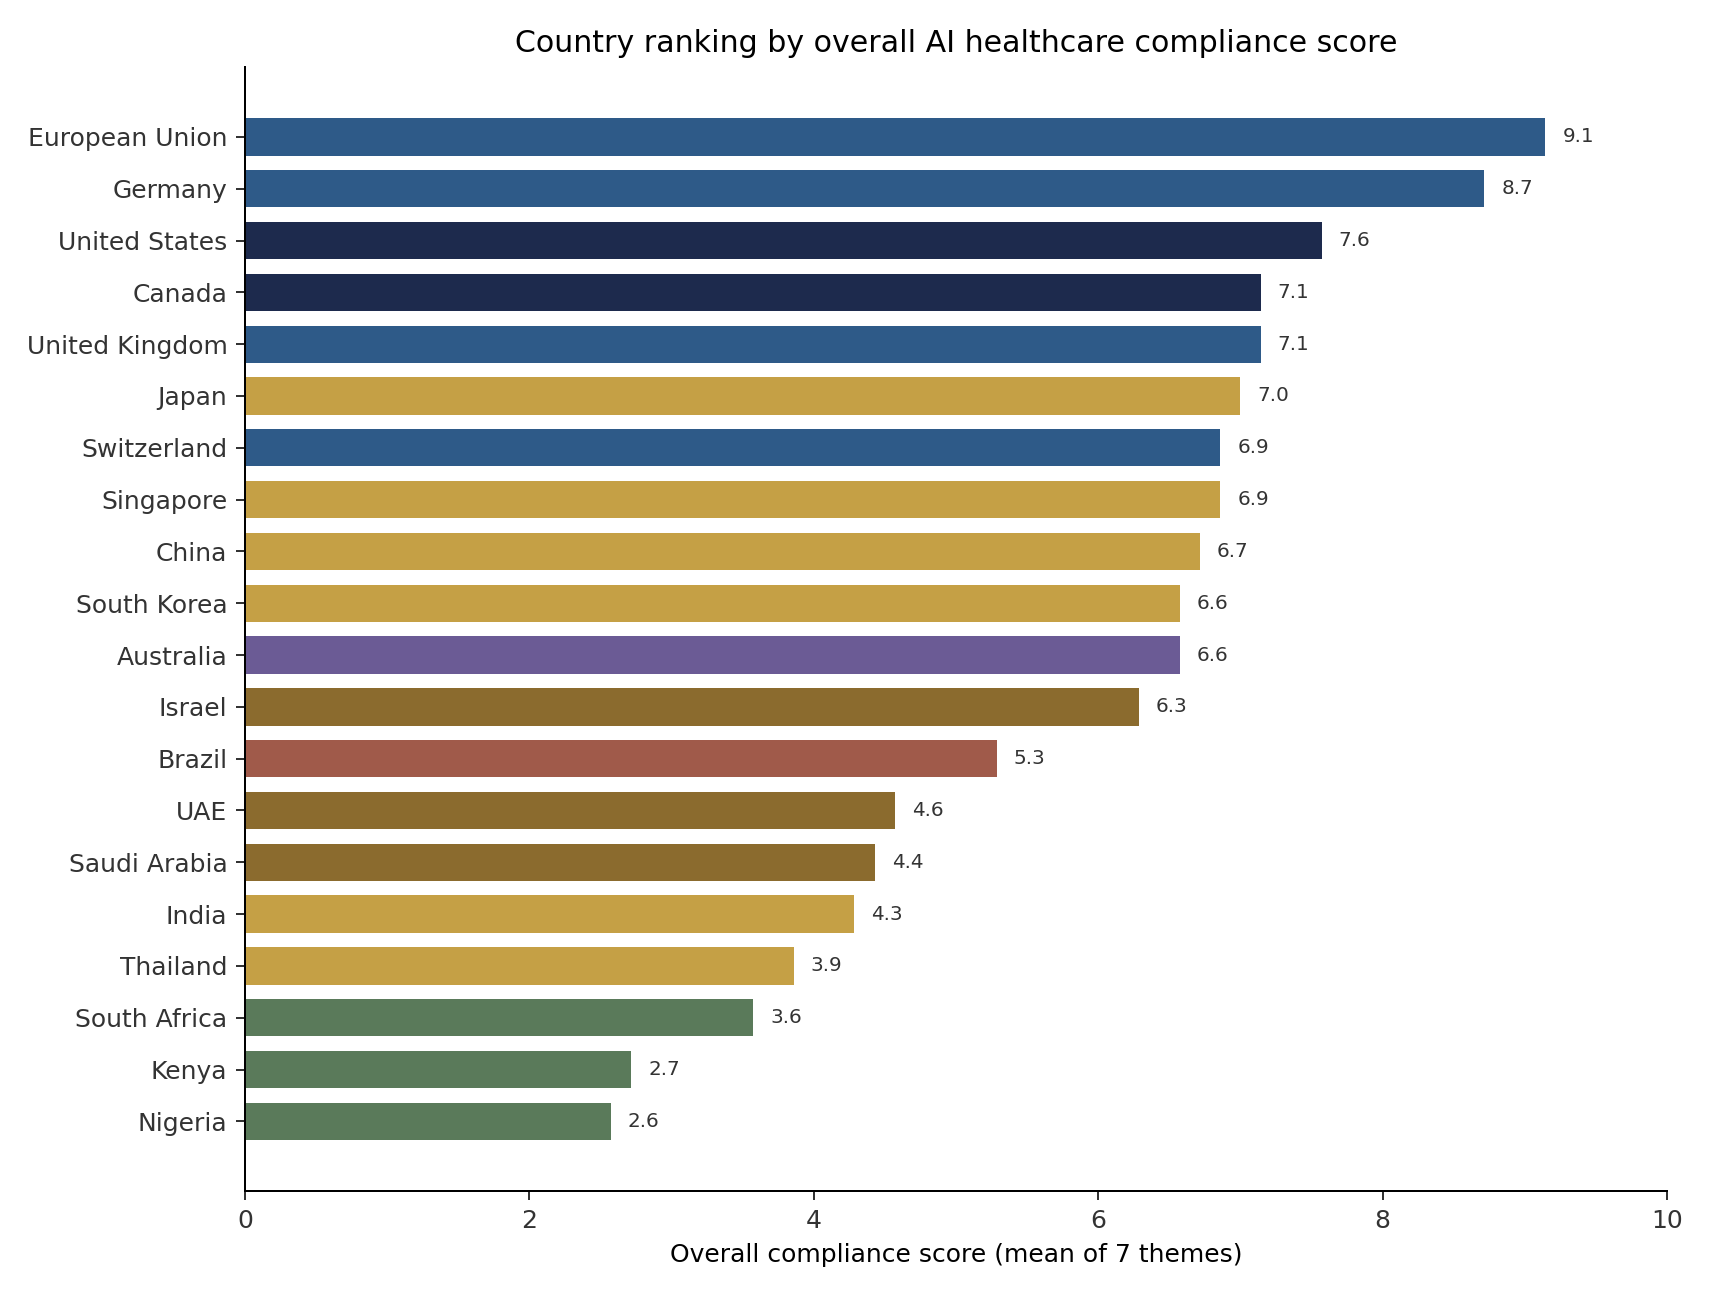
\includegraphics[width=0.82\textwidth]{figures/overall_ranking.png}
  \caption[Overall country ranking]{\textbf{Overall country ranking.} Each bar is the mean of the seven theme scores (1--10) for one jurisdiction. Bars are coloured by region. Longer bars mean stronger documented AI healthcare compliance. Read from bottom (highest) to top (lowest): the EU, Germany, and the United States lead; Kenya and Nigeria trail. Use this figure to show the jury the global spread of regulatory maturity at a glance.}
  \label{fig:overall-ranking}
\end{figure}

Table~\ref{tab:country-scores} provides the full theme-by-theme matrix used by the dashboard. Privacy = Data Privacy; Clin.\ = Clinical Validation; Appr.\ = Approval Process; Trans.\ = Transparency; Eth.\ = Ethics; Post = Post-Market; Liab.\ = Liability; Devices = reported AI device approvals (indicative counts).

{\footnotesize\setlength{\tabcolsep}{2.4pt}
\begin{longtable}{@{}l l l c c c c c c c c@{}}
\caption[Country compliance scores]{Country compliance scores (1--10) across seven themes} \label{tab:country-scores} \\
\toprule
\textbf{Country} & \textbf{Region} & \textbf{Maturity} & \textbf{Priv.} & \textbf{Clin.} & \textbf{Appr.} & \textbf{Trans.} & \textbf{Eth.} & \textbf{Post} & \textbf{Liab.} & \textbf{Devices} \\
\midrule
\endfirsthead
\toprule
\textbf{Country} & \textbf{Region} & \textbf{Maturity} & \textbf{Priv.} & \textbf{Clin.} & \textbf{Appr.} & \textbf{Trans.} & \textbf{Eth.} & \textbf{Post} & \textbf{Liab.} & \textbf{Devices} \\
\midrule
\endhead
\bottomrule
\endfoot
European Union & Europe & Advanced & 10 & 9 & 9 & 9 & 10 & 9 & 8 & 600 \\
Germany & Europe & Advanced & 10 & 9 & 9 & 8 & 9 & 9 & 7 & 180 \\
United States & North America & Advanced & 8 & 9 & 9 & 6 & 6 & 8 & 7 & 950 \\
United Kingdom & Europe & Advanced & 8 & 8 & 7 & 7 & 7 & 7 & 6 & 200 \\
Canada & North America & Advanced & 7 & 8 & 8 & 7 & 7 & 7 & 6 & 120 \\
Japan & Asia & Advanced & 7 & 8 & 8 & 6 & 7 & 8 & 5 & 150 \\
Singapore & Asia & Advanced & 7 & 7 & 7 & 8 & 8 & 6 & 5 & 60 \\
Switzerland & Europe & Advanced & 8 & 8 & 8 & 6 & 6 & 7 & 5 & 90 \\
China & Asia & Advanced & 7 & 7 & 7 & 7 & 6 & 7 & 6 & 300 \\
Australia & Oceania & Moderate & 7 & 7 & 7 & 6 & 7 & 7 & 5 & 80 \\
South Korea & Asia & Advanced & 7 & 7 & 8 & 6 & 6 & 7 & 5 & 200 \\
Israel & Middle East & Advanced & 6 & 8 & 7 & 6 & 6 & 6 & 5 & 100 \\
Brazil & South America & Developing & 7 & 5 & 5 & 5 & 5 & 5 & 5 & 40 \\
UAE & Middle East & Emerging & 5 & 5 & 5 & 5 & 5 & 4 & 3 & 35 \\
Saudi Arabia & Middle East & Emerging & 5 & 4 & 5 & 5 & 5 & 4 & 3 & 25 \\
India & Asia & Developing & 5 & 4 & 4 & 4 & 5 & 4 & 4 & 30 \\
Thailand & Asia & Developing & 5 & 4 & 4 & 4 & 4 & 3 & 3 & 15 \\
South Africa & Africa & Emerging & 6 & 3 & 3 & 3 & 4 & 3 & 3 & 10 \\
Kenya & Africa & Early & 5 & 2 & 3 & 2 & 3 & 2 & 2 & 3 \\
Nigeria & Africa & Early & 4 & 2 & 3 & 2 & 3 & 2 & 2 & 5 \\
\end{longtable}
}

\section{Theme-level comparison}

Figures~\ref{fig:theme-averages} and~\ref{fig:theme-gaps} and Table~\ref{tab:theme-leaders} answer two questions: which themes are strongest worldwide on average, and where countries diverge the most. A large gap means a divergence zone---some jurisdictions already have detailed AI rules, while others have almost none. Clinical validation and transparency show particularly wide spreads, which matters for multi-country evidence packages.

\begin{figure}[!htbp]
  \centering
  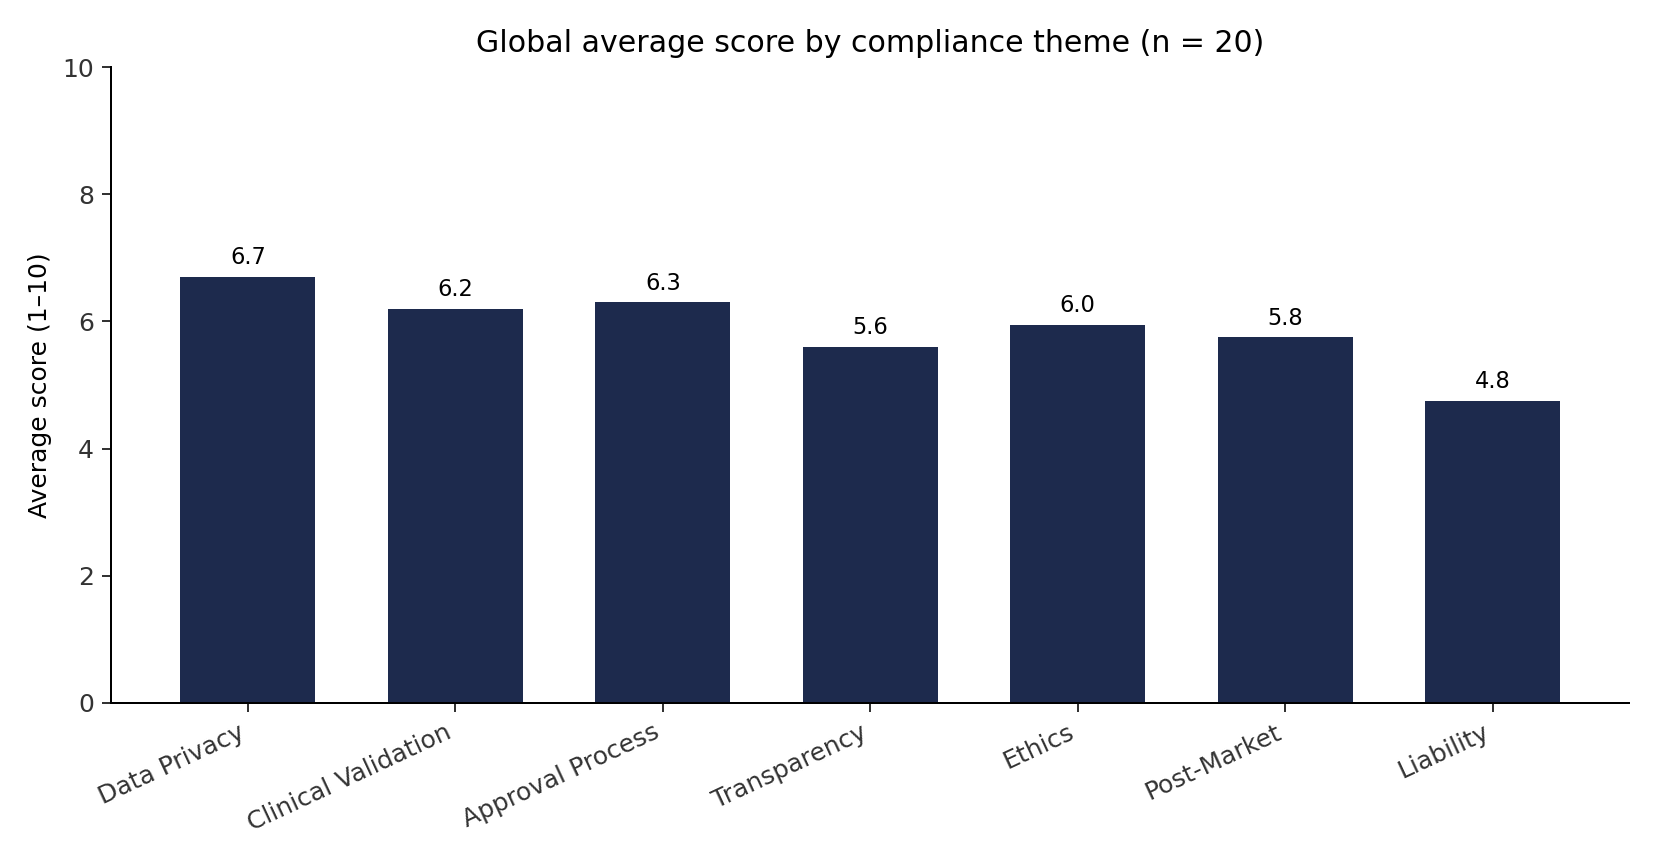
\includegraphics[width=0.88\textwidth]{figures/theme_averages.png}
  \caption[Global average score by theme]{\textbf{Global average score by theme.} For each of the seven compliance themes, the bar shows the mean score across all 20 countries. Higher bars mean that theme is more mature worldwide. Approval process and data privacy tend to lead (device pathways and post-GDPR privacy laws are widespread). Post-market surveillance and liability tend to lag, showing that lifecycle governance and accountability remain the weakest global pillars.}
  \label{fig:theme-averages}
\end{figure}

\begin{figure}[!htbp]
  \centering
  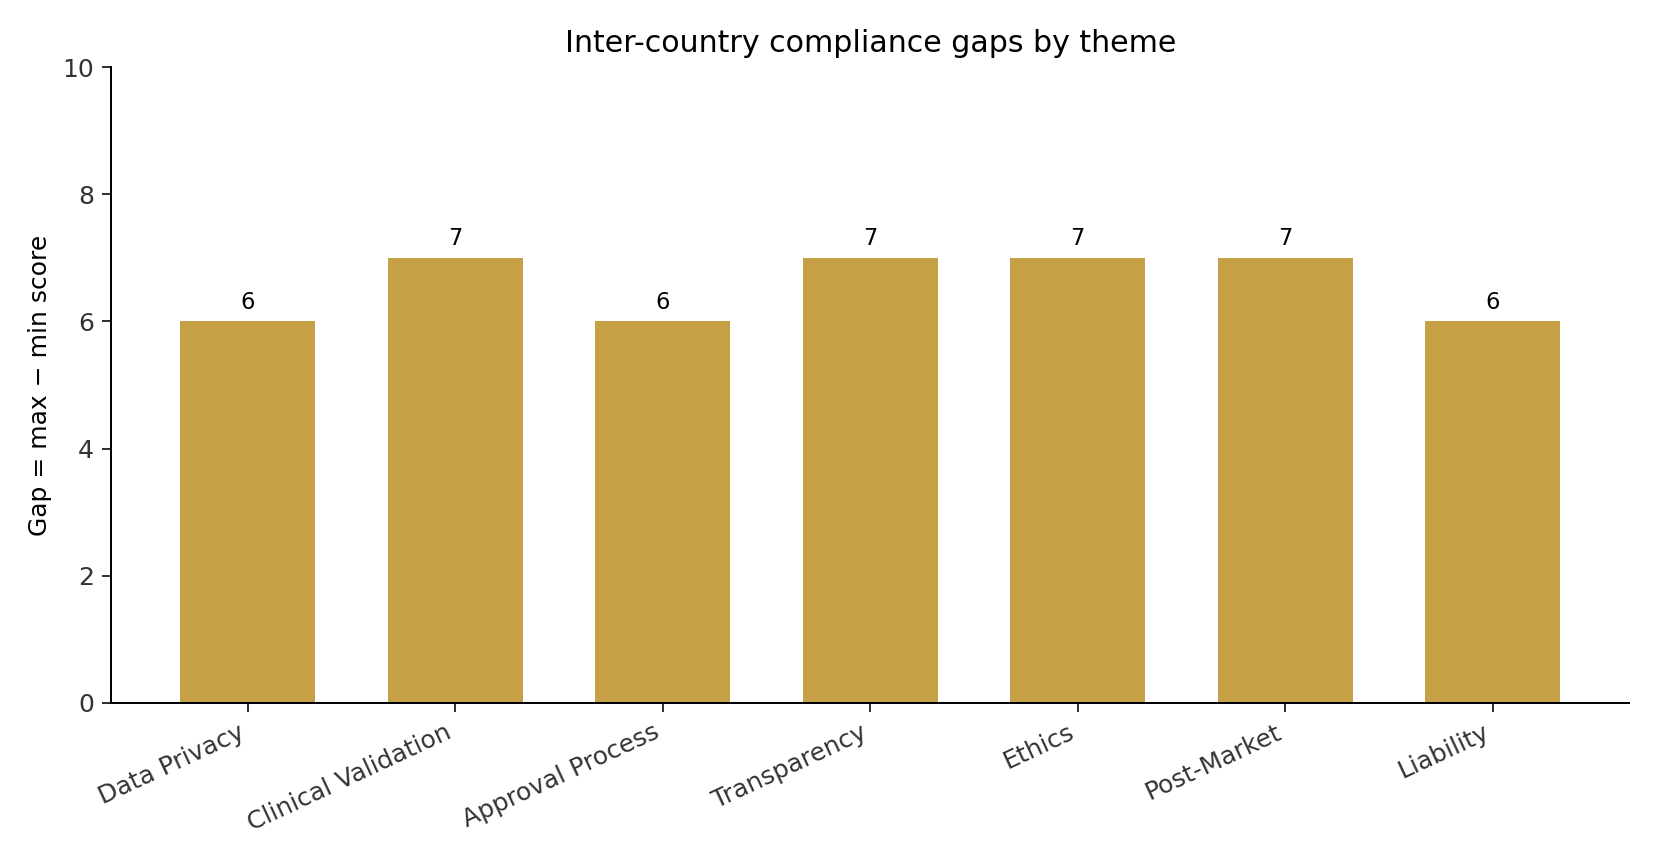
\includegraphics[width=0.88\textwidth]{figures/theme_gaps.png}
  \caption[Inter-country gaps by theme]{\textbf{Inter-country gaps by theme.} Gap $=$ maximum country score minus minimum country score for that theme. A large gap means strong divergence: some countries have detailed AI rules while others have almost none. Clinical validation and transparency typically show the widest gaps---important for developers who need multi-country evidence packages.}
  \label{fig:theme-gaps}
\end{figure}

\begin{table}[htbp]
\centering
\caption[Theme leaders and laggards]{Theme leaders and laggards across the 20-country sample}
\label{tab:theme-leaders}
\begin{tabular}{@{}l c l l@{}}
\toprule
\textbf{Theme} & \textbf{Gap} & \textbf{Leader} & \textbf{Laggard} \\
\midrule
Data Privacy & 6 & European Union & Nigeria \\
Clinical Validation & 7 & United States & Nigeria \\
Approval Process & 6 & United States & South Africa \\
Transparency & 7 & European Union & Nigeria \\
Ethics & 7 & European Union & Nigeria \\
Post-Market & 7 & European Union & Nigeria \\
Liability & 6 & European Union & Nigeria \\
\bottomrule
\end{tabular}
\end{table}


\subsection{How to read the theme leaders and laggards}

Table~\ref{tab:theme-leaders} lists, for each theme, the highest-scoring jurisdiction (leader), the lowest-scoring jurisdiction (laggard), and the numeric gap between them. The pattern is consistent and easy to summarise:

\begin{itemize}
  \item \textbf{Europe leads on rights and accountability themes.} The EU (and European peers) top data privacy, transparency, ethics, post-market, and liability. That reflects binding instruments---notably GDPR and the EU AI Act---rather than voluntary ethics checklists alone \cite{euaiact2024}.
  \item \textbf{The United States leads on market-access themes.} The US tops clinical validation and approval process, driven by FDA SaMD pathways, published authorisation counts, and related clinical evidence practice \cite{fda2021,wu2021}.
  \item \textbf{Early African jurisdictions dominate the laggard column.} Nigeria (and South Africa on approval process) appear repeatedly at the bottom. Device pathways and AI-specific adverse-event infrastructure are still forming there, so scores stay low even when privacy statutes exist.
\end{itemize}

In short: advanced regulators pull ahead where either enforceable privacy/ethics law or deep device pathways already exist; the largest gaps appear where those institutions are still early.

\section{Maturity distribution}

Figure~\ref{fig:maturity-mix} shows the frequency of maturity classes. Most jurisdictions in the sample are labelled \textbf{Advanced}, reflecting deliberate selection of major regulators alongside emerging markets. The smaller Early / Emerging / Developing groups are analytically important: they define the lower bound against which gaps are measured and they are the primary audience for capacity-building recommendations. Figure~\ref{fig:regional-overall} summarises mean overall scores by region.

\begin{figure}[!htbp]
  \centering
  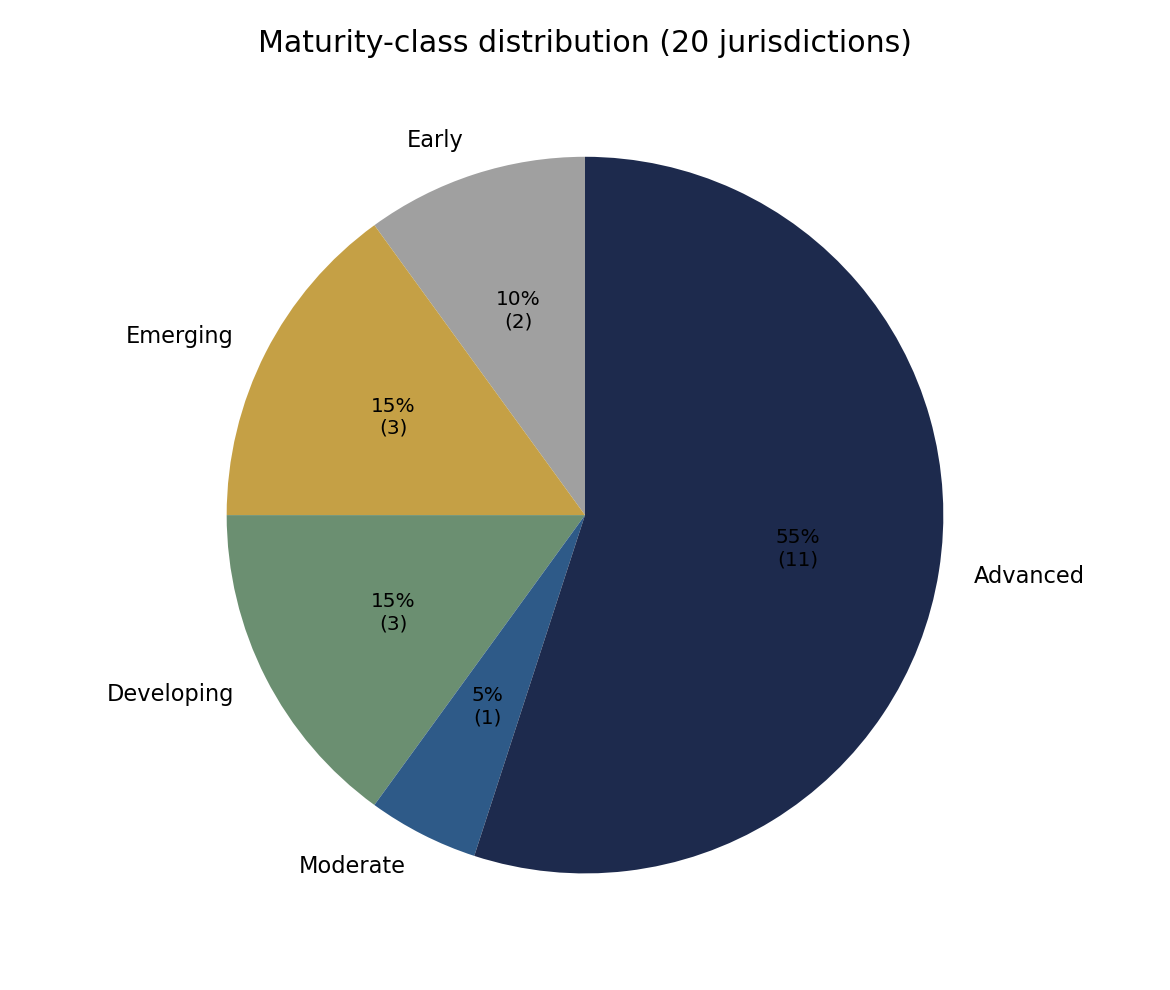
\includegraphics[width=0.72\textwidth]{figures/maturity_mix.png}
  \caption[Maturity-class distribution]{\textbf{Maturity-class distribution.} Pie slices show how many of the 20 jurisdictions fall into each qualitative maturity class (Early, Emerging, Developing, Moderate, Advanced). Maturity is assigned from documentary evidence (AI-specific rules, device pathway, approval activity, privacy/ethics enforcement)---not from a hidden formula on the scores alone. The Advanced slice is large because the sample deliberately includes major regulators; Early/Emerging countries define the capacity gap.}
  \label{fig:maturity-mix}
\end{figure}

\begin{figure}[!htbp]
  \centering
  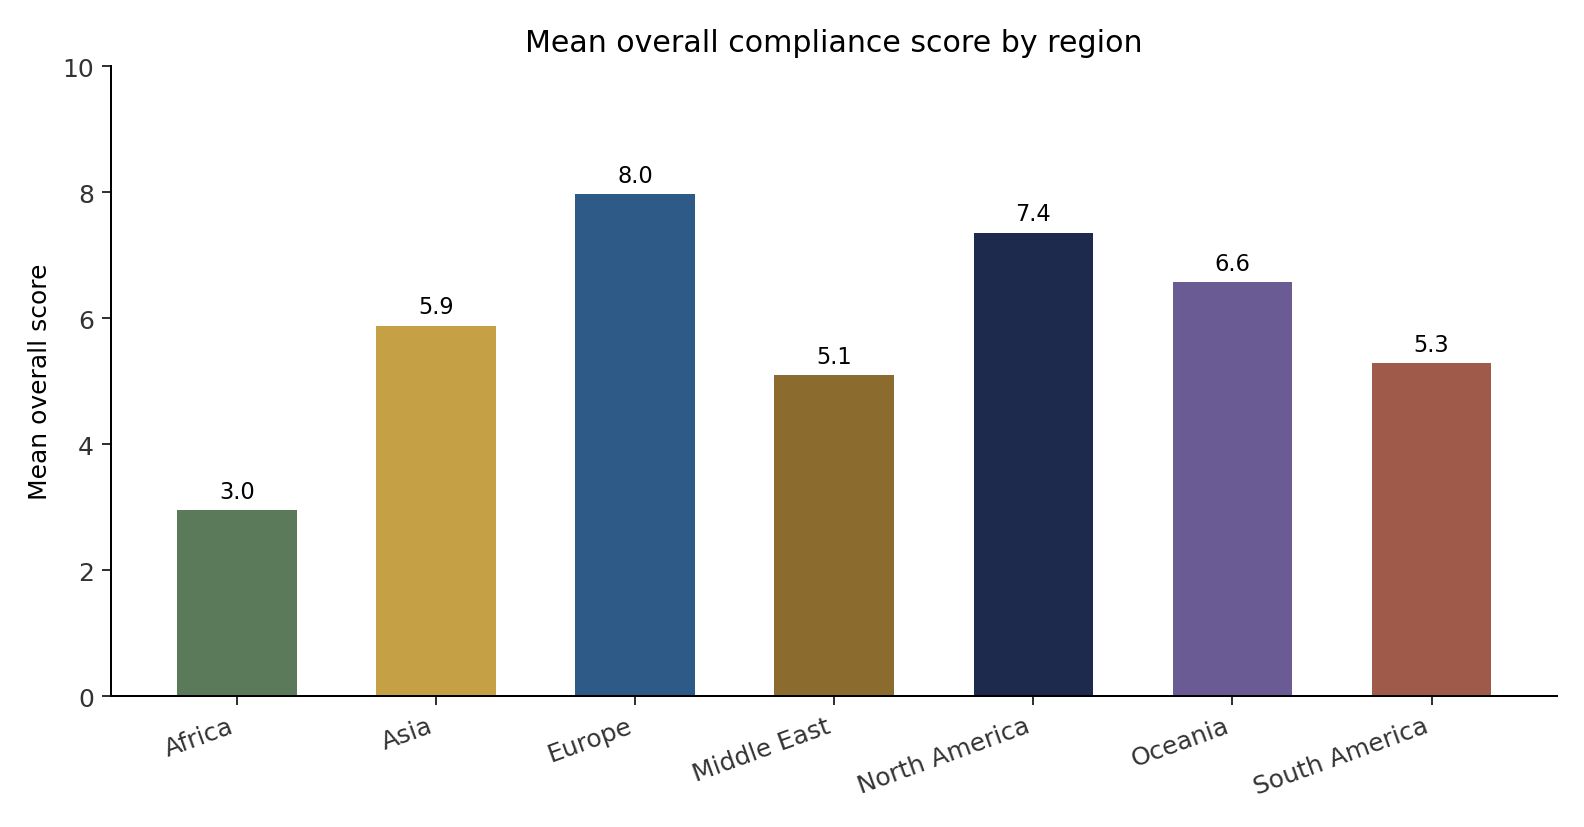
\includegraphics[width=0.88\textwidth]{figures/regional_overall.png}
  \caption[Mean overall compliance score by region]{\textbf{Mean overall compliance score by region.} Each bar is the average of country overall scores inside that region. Europe leads, followed by North America and Oceania; Africa is lowest. Asia sits in the middle because high performers (Japan, Singapore, South Korea, China) are averaged with developing pathways (India, Thailand). Oceania and South America rest on single-country observations (Australia, Brazil) and should not be over-generalised.}
  \label{fig:regional-overall}
\end{figure}

Maturity is not a hidden transform of the overall score. For example, China and Israel are Advanced despite mid-range privacy or liability scores, because they operate dedicated AI/device pathways with non-trivial approval activity. Australia is Moderate despite solid theme averages, reflecting a functioning but less AI-specialised pathway relative to FDA/EU peers.

\section{Regional comparative analysis}

Table~\ref{tab:regional-means} and Figures~\ref{fig:regional-overall}--\ref{fig:regional-heatmap} summarise regional means. Europe leads on the composite, followed by North America and Oceania; Africa trails substantially. Asia's mean sits in the middle because high performers (Japan, Singapore, South Korea, China) are averaged with developing pathways (India, Thailand).

\begin{table}[htbp]
\centering
\caption[Regional mean scores]{Regional mean scores and sample size}
\label{tab:regional-means}
\footnotesize
\setlength{\tabcolsep}{3.5pt}
\begin{tabular}{@{}l c c c c c c c c c@{}}
\toprule
\textbf{Region} & \textbf{n} & \textbf{Overall} & \textbf{Priv.} & \textbf{Clin.} & \textbf{Appr.} & \textbf{Trans.} & \textbf{Eth.} & \textbf{Post} & \textbf{Liab.} \\
\midrule
Africa & 3 & 3.0 & 5.0 & 2.3 & 3.0 & 2.3 & 3.3 & 2.3 & 2.3 \\
Asia & 6 & 5.9 & 6.3 & 6.2 & 6.3 & 5.8 & 6.0 & 5.8 & 4.7 \\
Europe & 4 & 8.0 & 9.0 & 8.5 & 8.2 & 7.5 & 8.0 & 8.0 & 6.5 \\
Middle East & 3 & 5.1 & 5.3 & 5.7 & 5.7 & 5.3 & 5.3 & 4.7 & 3.7 \\
North America & 2 & 7.4 & 7.5 & 8.5 & 8.5 & 6.5 & 6.5 & 7.5 & 6.5 \\
Oceania & 1 & 6.6 & 7.0 & 7.0 & 7.0 & 6.0 & 7.0 & 7.0 & 5.0 \\
South America & 1 & 5.3 & 7.0 & 5.0 & 5.0 & 5.0 & 5.0 & 5.0 & 5.0 \\
\bottomrule
\end{tabular}
\end{table}


\begin{figure}[!htbp]
  \centering
  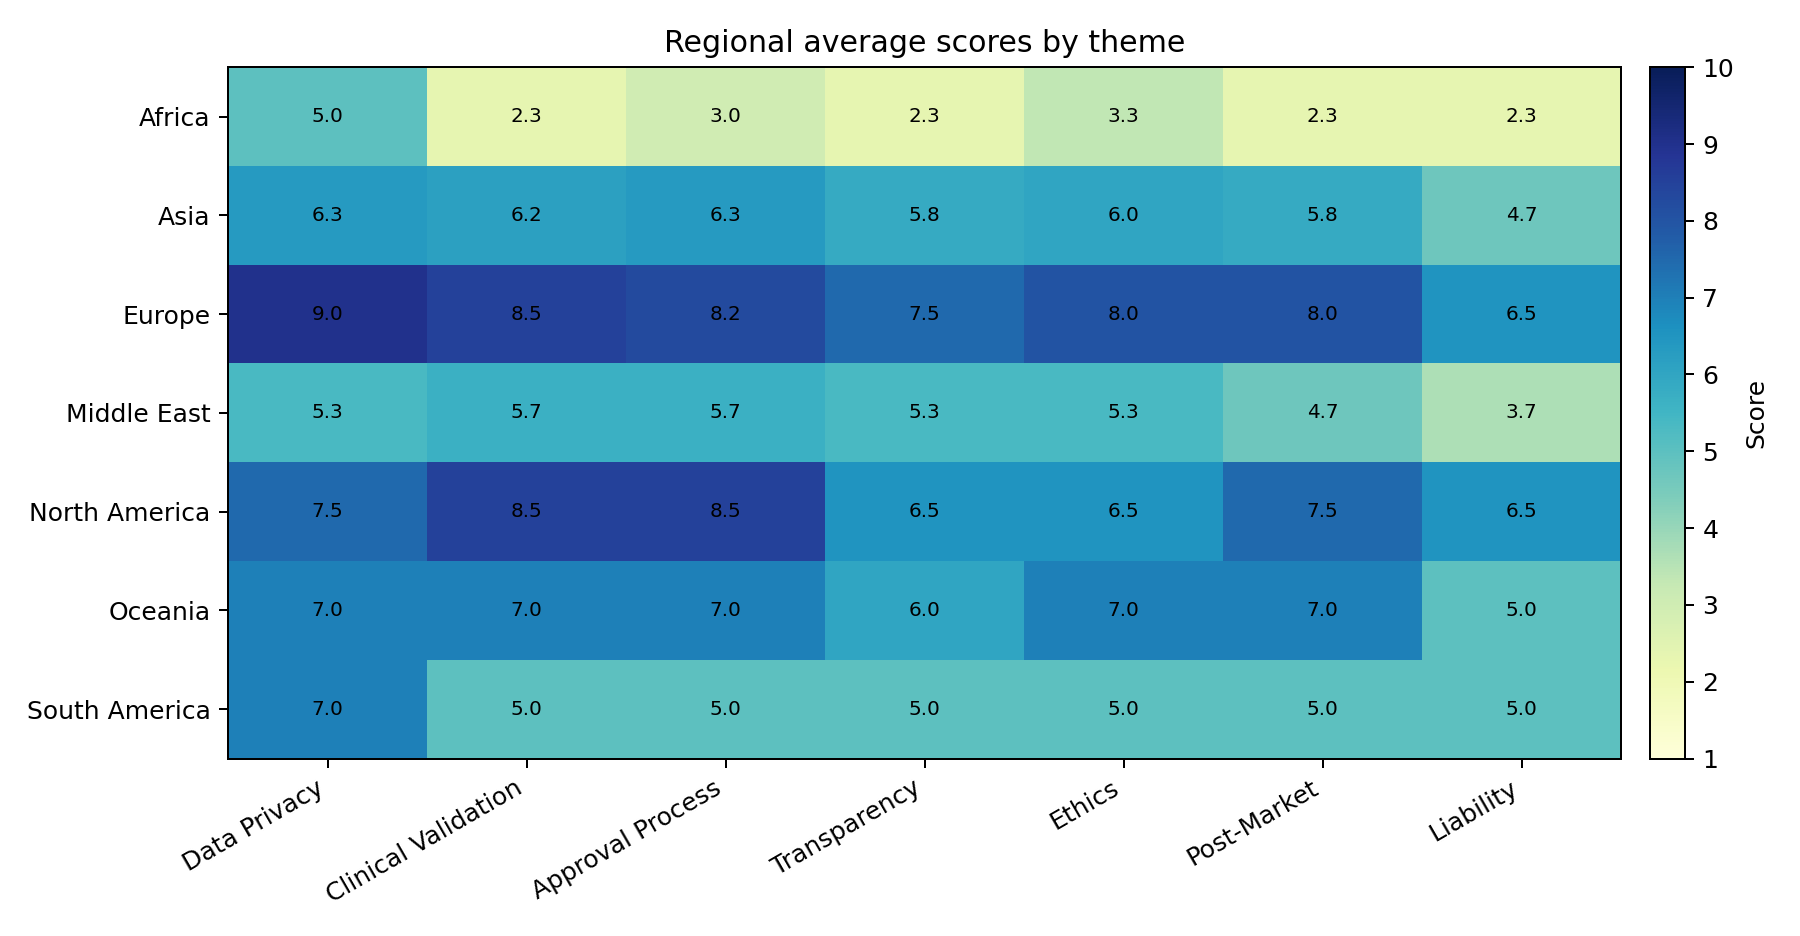
\includegraphics[width=0.92\textwidth]{figures/regional_heatmap.png}
  \caption[Regional theme heatmap]{\textbf{Regional theme heatmap.} Rows are regions; columns are the seven compliance themes. Cell colour and number show the regional mean score (darker $=$ higher). Read across a row to see a region's strengths/weaknesses; read down a column to see which region leads a theme. Europe is strong across privacy/ethics; North America is strong on clinical validation and approval; Africa shows low values on most AI-specific themes despite privacy progress in some countries.}
  \label{fig:regional-heatmap}
\end{figure}

\subsection{North America}
The United States and Canada are both Advanced. The US leads on approval process and clinical validation (FDA pathways plus PCCP) but is weaker on binding transparency and federal ethics law; HIPAA is sectoral rather than GDPR-equivalent \cite{cohen2018}. Canada pairs Health Canada device classes with closer GMLP alignment. North America offers high market-access volume with careful multi-state privacy mapping.

\subsection{Europe}
The EU aggregate, Germany, the United Kingdom, and Switzerland form the densest high-compliance cluster. The EU AI Act adds a binding high-risk layer on MDR SaMD and GDPR, lifting ethics and transparency relative to voluntary NIST-style frameworks \cite{euaiact2024}. Europe is the reference region for rights-based AI healthcare governance.

\subsection{Asia}
Asia is the most internally diverse region. Japan and Singapore combine mature agencies with structured AI guidance; South Korea and China show high approval throughput and algorithm-specific rules \cite{nmpa2021,pmda2020}. India and Thailand remain Developing: medical-device frameworks exist, but AI-specific validation and post-market duties are thinner. Cross-border AI deployment in Asia cannot assume a single evidence package.

\subsection{Middle East, Africa, Oceania, and South America}
Israel is Advanced (innovation- and device-driven). Saudi Arabia and the UAE are Emerging (strategy-led catch-up). In Africa, South Africa (POPIA, Emerging) outranks Kenya and Nigeria (Early): data-protection progress outpaces AI-device infrastructure. Australia (Moderate) offers a functioning TGA pathway; Brazil (Developing) is privacy-strong (LGPD) relative to clinical-validation scores.

\section{Peer jurisdiction comparison}

Figure~\ref{fig:peer-comparison} compares five representative jurisdictions side by side across all seven themes: the United States and the European Union (Advanced leaders), China (Advanced Asian regulator with high approval activity), India (Developing), and South Africa (Emerging). Figure~\ref{fig:radar-top5} complements this by showing radar shapes for the five highest overall scorers.

\begin{figure}[!htbp]
  \centering
  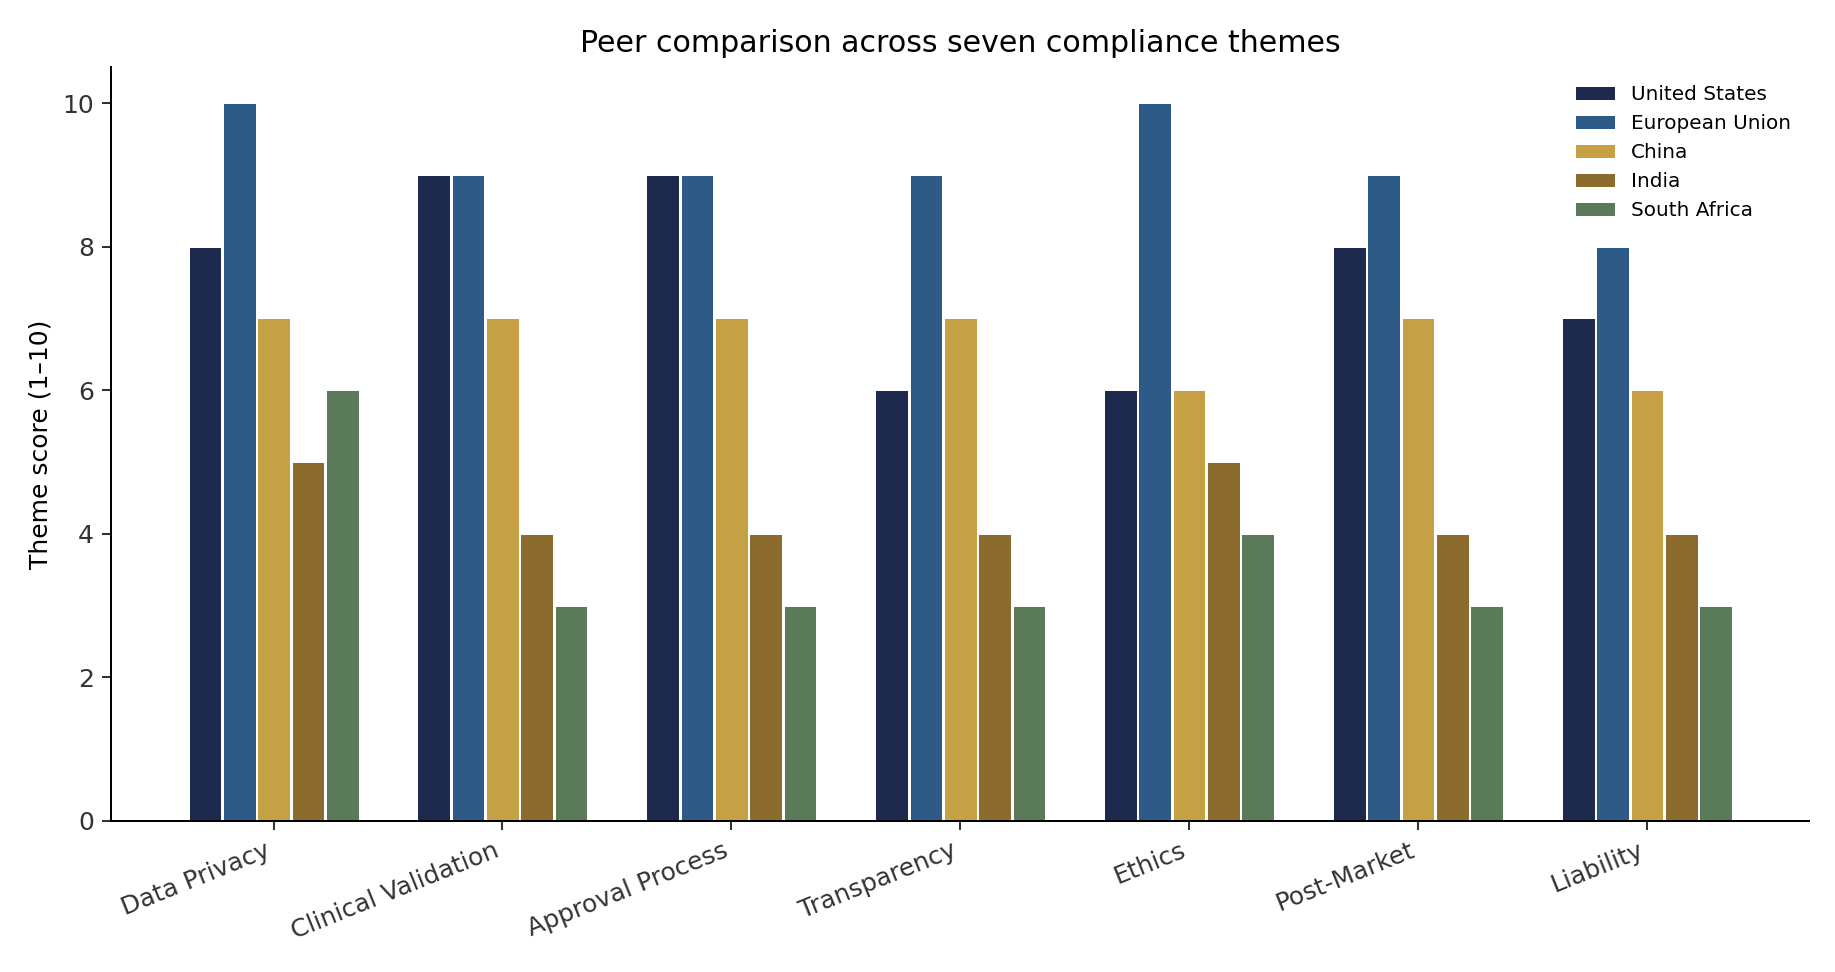
\includegraphics[width=0.95\textwidth]{figures/peer_comparison.png}
  \caption[Peer comparison across seven themes]{\textbf{Peer comparison across seven themes.} Grouped bars compare the United States, European Union, China, India, and South Africa on each compliance theme (score 1--10). Read theme by theme: the US and EU are high on most axes, with the EU typically stronger on privacy/ethics/transparency and the US strong on clinical validation and approval. China is competitive on approval and mid-range on privacy. India and South Africa sit lower, especially on clinical validation, post-market, and liability---illustrating the Advanced vs Developing/Emerging gap in one chart.}
  \label{fig:peer-comparison}
\end{figure}

\begin{figure}[!htbp]
  \centering
  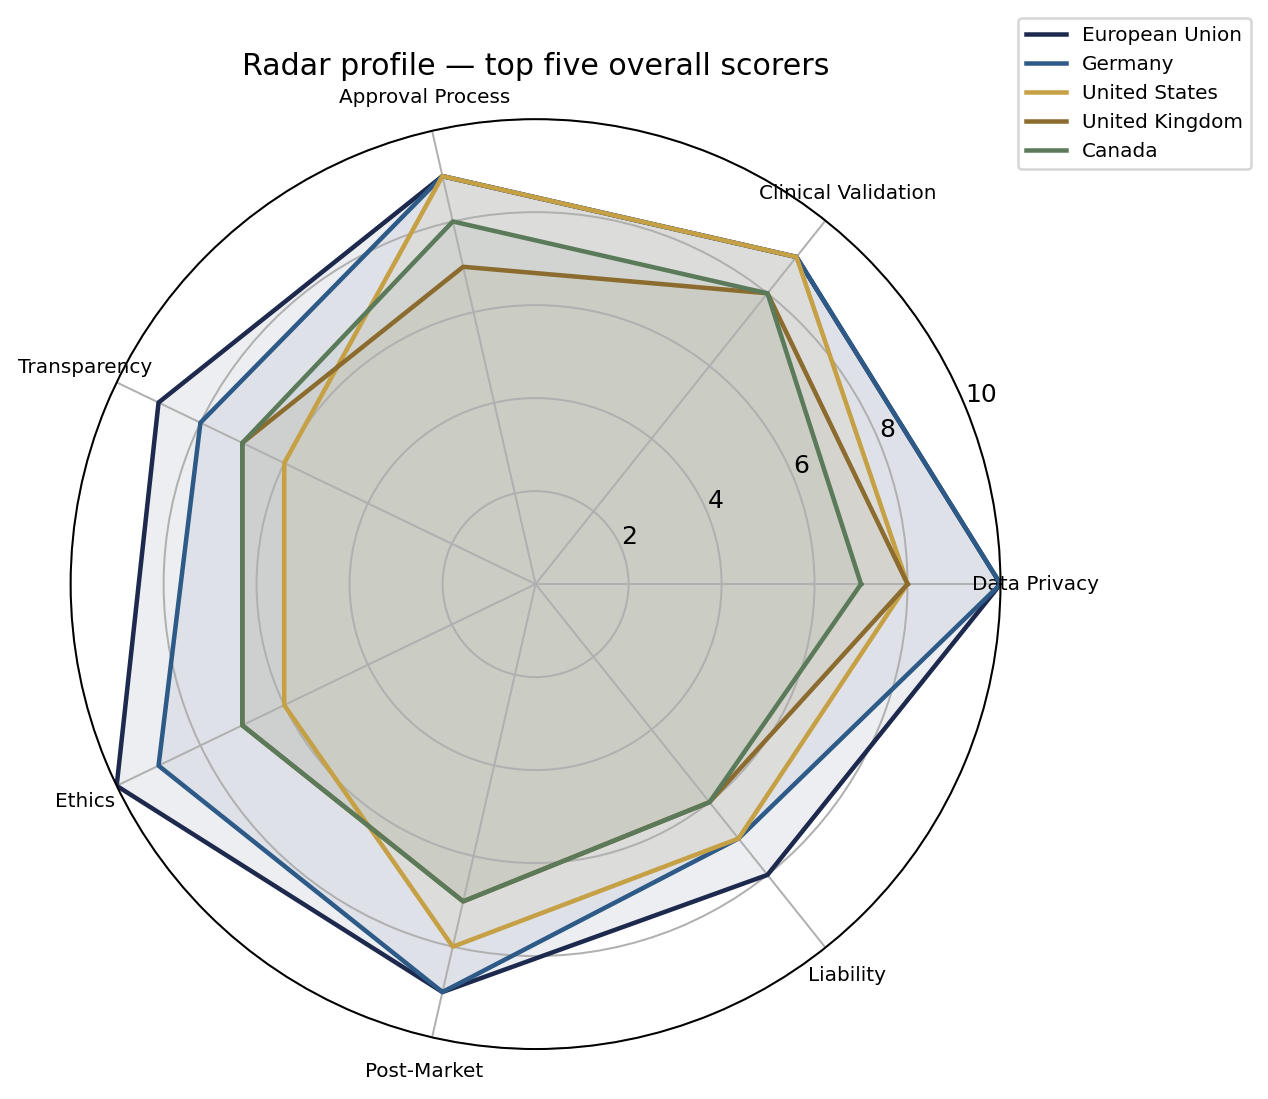
\includegraphics[width=0.78\textwidth]{figures/radar_top5.png}
  \caption[Radar profiles of the top five scorers]{\textbf{Radar profiles of the top five scorers;} Each coloured polygon is one top jurisdiction across the seven themes (axes from centre 0 to outer rim 10). A wider polygon means stronger scores. Compare shapes: EU/Germany typically extend farthest on privacy and ethics; the United States extends farthest on clinical validation and approval process, with a relative dip on transparency/ethics. This shows that ``best country'' depends on which theme matters for the product.}
  \label{fig:radar-top5}
\end{figure}

\section{Pairwise and strategic comparisons}

\paragraph{United States vs.\ European Union:}
Both are Advanced. The US offers speed and volume through established SaMD pathways and PCCP for adaptive algorithms \cite{fda2023}. The EU offers stricter enforceable transparency, ethics, and privacy duties under GDPR + AI Act + MDR. A dual-track strategy (US clinical evidence + EU conformity/quality system) remains common for global SaMD vendors \cite{muehlematter2021}.

\paragraph{China vs.\ Japan:}
Both are Advanced Asian regulators with distinct emphases: China emphasises registration guidance and domestic algorithm filing practices; Japan emphasises PMDA DASH evaluation and quality-system discipline. Privacy scores are similar; liability remains a shared soft spot relative to Europe.

\paragraph{Singapore vs.\ India:}
Singapore's Advanced governance (clear guidance, sandbox culture, strong ethics/transparency relative to region) contrasts with India's Developing trajectory (large digital-health ambition, DPDP privacy progress, thinner AI-device clinical pathway). For ASEAN-oriented products, Singapore is often the regional reference; India is a scale market requiring staged compliance investment.

\paragraph{Israel vs.\ Gulf states:}
Israel's Advanced profile is innovation- and device-driven. Saudi Arabia and the UAE are investment- and strategy-driven Emerging systems: scores are mid-low today, but national AI agendas imply rapid movement if pathways and surveillance infrastructure catch up.

\paragraph{South Africa vs.\ Kenya / Nigeria:}
Within Africa, South Africa's POPIA-era privacy and relatively stronger institutions produce a clearer Emerging profile. Kenya and Nigeria remain Early on clinical validation, transparency, and post-market themes despite recent data-protection statutes---illustrating that privacy law alone does not raise overall healthcare-AI compliance.

\section{Country-by-country profiles}

The following compact profiles, ordered by overall score, summarise each jurisdiction. They are the narrative counterpart of the dashboard Country Details page and should be read with Tables~\ref{tab:overall-rank} and~\ref{tab:country-scores}.

{\footnotesize
\begin{description}[style=unboxed,leftmargin=0.6cm,font=\normalfont\bfseries]

\item[European Union] Europe; Advanced; overall 9.1/10; European Medicines Agency (EMA), National Competent Authorities, Notified Bodies; 600 devices; first AI instrument 2018. Scores: P10 C9 A9 T9 E10 PM9 L8. Privacy: GDPR (General Data Protection Regulation). AI rule: EU AI Act (2024). Challenges: Complex multi-layered regulatory landscape. Harmonization across 27 member states. Notified Body capacity constraints. Risk of over-regulation stifling innov... Notable: EU AI Act is the world's first comprehensive AI law. High-risk healthcare AI must comply by 2026-2027. EHDS aims to create a unified health data framework.
\item[Germany] Europe; Advanced; overall 8.7/10; BfArM (Federal Institute for Drugs and Medical Devices); 180 devices; first AI instrument 2018. Scores: P10 C9 A9 T8 E9 PM9 L7. Privacy: GDPR + BDSG (Federal Data Protection Act). AI rule: EU AI Act (as EU member). National AI Strategy (2018, updated 2020).. Challenges: Historically strict data protection culture can slow health data utilization. DiGA program growing pains. Interoperability of health IT systems. Notable: DiGA is the world's first regulatory pathway for prescribed digital therapies reimbursed by statutory health insurance. Health Data Use Act aims to unlock re...
\item[United States] North America; Advanced; overall 7.6/10; FDA (Food and Drug Administration); 950 devices; first AI instrument 2017. Scores: P8 C9 A9 T6 E6 PM8 L7. Privacy: HIPAA (Health Insurance Portability and Accountability Act). AI rule: FDA AI/ML-Based SaMD Action Plan (2021). Challenges: Fragmented state-level privacy laws. No comprehensive federal AI legislation. Balancing innovation speed with safety oversight for adaptive algorithms. Notable: FDA has authorized over 950 AI/ML-enabled medical devices as of 2025. Predetermined Change Control Plan allows manufacturers to pre-specify algorithm modific...
\item[United Kingdom] Europe; Advanced; overall 7.1/10; MHRA (Medicines and Healthcare products Regulatory Agency); 200 devices; first AI instrument 2018. Scores: P8 C8 A7 T7 E7 PM7 L6. Privacy: UK GDPR \& Data Protection Act 2018. AI rule: Pro-innovation AI Regulation Framework (2023). Challenges: Post-Brexit regulatory divergence from EU. Balancing light-touch innovation-friendly approach with patient safety. Transition from CE to UKCA marking. Notable: UK positioned as pro-innovation alternative to EU AI Act. AI Safety Institute is a world-first government body for AI safety research. NHS AI Lab supports AI...
\item[Canada] North America; Advanced; overall 7.1/10; Health Canada; 120 devices; first AI instrument 2019. Scores: P7 C8 A8 T7 E7 PM7 L6. Privacy: PIPEDA (Personal Information Protection and Electronic Documents Act), Provincial health privacy laws (e.g., Ontario PHIPA). AI rule: AIDA (Artificial Intelligence and Data Act, proposed in Bill C-27). Challenges: Federal-provincial jurisdiction complexity. AIDA legislation delayed. Keeping pace with rapid AI advancement in healthcare. Notable: Canada co-developed GMLP with FDA and MHRA. Pan-Canadian Health Data Strategy in development. Strong AI research ecosystem (MILA, Vector, Amii) informing pol...
\item[Japan] Asia; Advanced; overall 7.0/10; PMDA (Pharmaceuticals and Medical Devices Agency); 150 devices; first AI instrument 2019. Scores: P7 C8 A8 T6 E7 PM8 L5. Privacy: APPI (Act on Protection of Personal Information, amended 2022). AI rule: AI Guidelines for Business (2024), Social Principles of Human-Centric AI (2019). Challenges: Aging society drives demand but conservative regulatory culture. Language barriers in international harmonization. Slow adoption of digital health relative t... Notable: Japan's regulatory sandbox (IDATEN) accelerates innovative device approval. Society 5.0 vision integrates AI in healthcare transformation. PMDA actively deve...
\item[Singapore] Asia; Advanced; overall 6.9/10; HSA (Health Sciences Authority); 60 devices; first AI instrument 2019. Scores: P7 C7 A7 T8 E8 PM6 L5. Privacy: PDPA (Personal Data Protection Act, 2012, amended 2021). AI rule: Model AI Governance Framework (2019, updated 2020), AI Verify (2022). Challenges: Small domestic market limits local clinical evidence generation. Balancing business-friendly environment with robust oversight. Regional influence vs. global... Notable: AI Verify is the world's first AI governance testing framework. Singapore positioned as AI governance thought leader in ASEAN. Strong public-private partners...
\item[Switzerland] Europe; Advanced; overall 6.9/10; Swissmedic; 90 devices; first AI instrument 2023. Scores: P8 C8 A8 T6 E6 PM7 L5. Privacy: nFADP (New Federal Act on Data Protection, 2023). AI rule: No AI-specific law. Federal Council AI guidelines. Bilateral alignment with EU standards.. Challenges: Dependency on EU regulatory decisions without EU membership voting rights. Maintaining bilateral agreements post-EU AI Act. Small market size. Notable: Strong pharma/medtech hub (Novartis, Roche). nFADP brings Swiss privacy law to GDPR-equivalent. Active AI health research at ETH Zurich and EPFL.
\item[China] Asia; Advanced; overall 6.7/10; NMPA (National Medical Products Administration); 300 devices; first AI instrument 2021. Scores: P7 C7 A7 T7 E6 PM7 L6. Privacy: PIPL (Personal Information Protection Law, 2021). AI rule: Interim Measures for Generative AI (2023), Algorithm Recommendation Regulations (2022), Deep Synthesis Regulations (2023). Challenges: Rapid regulatory evolution creates compliance complexity. Data localization requirements limit international collaboration. Balancing state surveillance prio... Notable: China is among the first to regulate algorithmic recommendations and generative AI. NMPA rapidly approving AI diagnostic tools. National AI standardization e...
\item[Australia] Oceania; Moderate; overall 6.6/10; TGA (Therapeutic Goods Administration); 80 devices; first AI instrument 2019. Scores: P7 C7 A7 T6 E7 PM7 L5. Privacy: Privacy Act 1988 (amended), Australian Privacy Principles (APPs). AI rule: Australia's AI Ethics Principles (2019), Voluntary AI Safety Standard (2024). Challenges: Voluntary nature of AI ethics framework limits enforcement. Resource constraints in TGA for AI evaluation. Geographic barriers to clinical trial recruitment. Notable: Australia's AI Ethics Principles among the earliest globally. TGA actively developing SaMD regulatory pathways. National Digital Health Strategy driving AI i...
\item[South Korea] Asia; Advanced; overall 6.6/10; MFDS (Ministry of Food and Drug Safety); 200 devices; first AI instrument 2019. Scores: P7 C7 A8 T6 E6 PM7 L5. Privacy: PIPA (Personal Information Protection Act, amended 2023). AI rule: AI Framework Act (proposed), National AI Strategy (2019). Challenges: Balancing rapid technological adoption with regulatory oversight. Harmonizing domestic standards with international frameworks. SME compliance burden. Notable: South Korea has one of the highest AI medical device approval rates globally. MFDS Regulatory Science Center is a dedicated AI device evaluation unit. K-BioH...
\item[Israel] Middle East; Advanced; overall 6.3/10; MOH AMAR (Division of Medical Devices, Ministry of Health); 100 devices; first AI instrument 2022. Scores: P6 C8 A7 T6 E6 PM6 L5. Privacy: Privacy Protection Law (1981, amended), Health Information Exchange regulations. AI rule: AI Policy and Ethics Framework (2022), National AI Program. Challenges: Outdated base privacy legislation. Balancing startup-friendly ecosystem with regulatory rigor. Small domestic market necessitates international focus. Notable: Israel is a global health AI innovation hub. Unique national health data infrastructure enables world-class AI research. Highest health AI startups per capit...
\item[Brazil] South America; Developing; overall 5.3/10; ANVISA (Agência Nacional de Vigilância Sanitária); 40 devices; first AI instrument 2020. Scores: P7 C5 A5 T5 E5 PM5 L5. Privacy: LGPD (Lei Geral de Proteção de Dados, 2020). AI rule: AI Bill (PL 2338/2023, under legislative process). Challenges: AI regulatory framework still in legislative process. Limited ANVISA capacity for AI device evaluation. Digital health infrastructure gaps in underserved reg... Notable: LGPD is Latin America's most comprehensive data protection law. Active AI legislation process. Growing health AI startup ecosystem in São Paulo.
\item[UAE] Middle East; Emerging; overall 4.6/10; MOH (Ministry of Health and Prevention), HAAD, DHA; 35 devices; first AI instrument 2017. Scores: P5 C5 A5 T5 E5 PM4 L3. Privacy: Federal Decree-Law No. 45/2021 (Personal Data Protection). AI rule: National AI Strategy 2031, Minister of State for AI appointed (2017). Challenges: Multi-authority regulatory landscape (federal and emirate-level). Rapid strategy ambitions vs. regulatory maturity. Building domestic healthcare data infrast... Notable: First country to appoint a Minister of State for AI (2017). Ambitious National AI Strategy 2031. Hub for health AI startups and international collaborations.
\item[Saudi Arabia] Middle East; Emerging; overall 4.4/10; SFDA (Saudi Food and Drug Authority); 25 devices; first AI instrument 2023. Scores: P5 C4 A5 T5 E5 PM4 L3. Privacy: PDPL (Personal Data Protection Law, 2023). AI rule: SDAIA AI Ethics Principles (2023), National AI Strategy. Challenges: Regulatory framework still maturing. Building domestic regulatory expertise. Dependency on international recognition pathways. Limited public health data inf... Notable: Massive AI investment under Vision 2030. SDAIA established as dedicated AI authority. NEOM project integrating AI healthcare. Rapid digital health transforma...
\item[India] Asia; Developing; overall 4.3/10; CDSCO (Central Drugs Standard Control Organisation); 30 devices; first AI instrument 2023. Scores: P5 C4 A4 T4 E5 PM4 L4. Privacy: Digital Personal Data Protection Act (DPDP, 2023). AI rule: No AI-specific law. NITI Aayog AI Strategy and Responsible AI guidelines (2021).. Challenges: Regulatory framework still maturing for AI devices. Limited CDSCO capacity for AI/ML evaluation. Infrastructure gaps in digital health. Balancing innovation ... Notable: DPDP Act 2023 is India's first comprehensive data protection law. Ayushman Bharat Digital Mission building foundational digital health infrastructure. IndiaA...
\item[Thailand] Asia; Developing; overall 3.9/10; Thai FDA (Food and Drug Administration); 15 devices; first AI instrument 2022. Scores: P5 C4 A4 T4 E4 PM3 L3. Privacy: PDPA (Personal Data Protection Act, 2022). AI rule: National AI Strategy and Action Plan (2022-2027). No binding AI law.. Challenges: Regulatory framework for AI devices still developing. Digital health infrastructure building. Balancing medical tourism innovation with domestic healthcare p... Notable: PDPA implementation is a major privacy milestone. Thailand 4.0 drives digital health investment. Medical tourism sector catalyzing AI adoption.
\item[South Africa] Africa; Emerging; overall 3.6/10; SAHPRA (South African Health Products Regulatory Authority); 10 devices; first AI instrument 2021. Scores: P6 C3 A3 T3 E4 PM3 L3. Privacy: POPIA (Protection of Personal Information Act, 2021). AI rule: No AI-specific regulation. AI Policy Framework under development.. Challenges: SAHPRA capacity and resource constraints. Digital infrastructure gaps. Brain drain in health AI expertise. Balancing innovation with addressing basic healthc... Notable: POPIA is Africa's most comprehensive data protection law. CSIR and universities driving AI health research. Growing health tech ecosystem in Cape Town and Jo...
\item[Kenya] Africa; Early; overall 2.7/10; PPB (Pharmacy and Poisons Board); 3 devices; first AI instrument 2019. Scores: P5 C2 A3 T2 E3 PM2 L2. Privacy: Data Protection Act (2019). AI rule: No AI-specific regulation. Blockchain and AI Taskforce Report (2019).. Challenges: Limited regulatory capacity. Infrastructure constraints. Prioritizing basic healthcare access alongside innovation. Dependency on international standards and... Notable: Kenya is a mobile health innovation leader in Africa. Data Protection Act among earliest in East Africa. Growing AI-for-health research at universities and t...
\item[Nigeria] Africa; Early; overall 2.6/10; NAFDAC (National Agency for Food and Drug Administration and Control); 5 devices; first AI instrument 2023. Scores: P4 C2 A3 T2 E3 PM2 L2. Privacy: NDPR (Nigeria Data Protection Regulation, 2019) / NDPA (Nigeria Data Protection Act, 2023). AI rule: National AI Strategy (draft). No binding AI regulation.. Challenges: Limited regulatory capacity for AI devices. Digital infrastructure gaps. Healthcare access challenges precede AI adoption. Funding constraints for regulatory... Notable: NDPA 2023 is a significant step in data governance. Growing AI research community (e.g., Data Science Nigeria). Mobile health innovations bypassing tradition...
\end{description}
}

\clearpage
\section{Global trends}

Table~\ref{tab:global-trends} records structured trend objects with adoption level, emergence year, and narrative description. Convergence does not mean identical laws; it means shared principles and similar instruments (risk-based SaMD classification, GDPR-style protection, GMLP, lifecycle / PCCP thinking, and a shift from voluntary ethics toward binding rules such as the EU AI Act).

\begin{tcolorbox}[
  colback=white,
  colframe=aivanavy,
  boxrule=0.9pt,
  arc=1.5pt,
  left=2pt,
  right=2pt,
  top=3pt,
  bottom=3pt,
  breakable,
]
\footnotesize
\setlength{\tabcolsep}{5pt}
\renewcommand{\arraystretch}{1.3}
\begin{longtable}{|>{\raggedright\arraybackslash}p{0.22\textwidth}|>{\raggedright\arraybackslash}p{0.48\textwidth}|>{\centering\arraybackslash}p{0.12\textwidth}|>{\centering\arraybackslash}p{0.08\textwidth}|}
\caption[Global trends in AI healthcare regulation]{Global trends in AI healthcare regulation} \label{tab:global-trends} \\
\hline
\rowcolor{aivagray}
\textbf{Trend} & \textbf{Description} & \textbf{Adoption} & \textbf{Since} \\
\hline
\endfirsthead
\hline
\rowcolor{aivagray}
\textbf{Trend} & \textbf{Description} & \textbf{Adoption} & \textbf{Since} \\
\hline
\endhead
\hline
\endfoot
Convergence on Risk-Based Regulation & Most jurisdictions adopting risk-based classification of AI medical devices, influenced by IMDRF framework. & High & 2017 \\ \hline
Comprehensive Data Protection Laws & Post-GDPR wave of national data protection laws with health data as sensitive category. & High & 2018 \\ \hline
AI-Specific Legislation & Growing trend toward dedicated AI laws (EU AI Act leading, followed by Brazil, Canada, South Korea proposals). & Medium & 2021 \\ \hline
International Harmonization Efforts & IMDRF, GMLP (FDA-Health Canada-MHRA), and WHO guidance driving convergence. & Medium & 2019 \\ \hline
Ethical AI Frameworks & Proliferation of national AI ethics principles, mostly voluntary, increasingly being legislated. & High & 2018 \\ \hline
Regulatory Sandboxes for Health AI & Controlled testing environments for innovative AI devices before full regulatory compliance. & Low & 2020 \\ \hline
Real-World Evidence Acceptance & Growing regulatory acceptance of real-world data and evidence for AI device evaluation. & Medium & 2019 \\ \hline
Adaptive Algorithm Governance & Frameworks for managing continuously learning AI systems (e.g., FDA Predetermined Change Control Plan). & Low & 2021 \\ \hline
AI Adoption in Radiology and Digital Pathology Workflows & AI image analysis is increasingly deployed for triage and decision support in radiology and pathology, driving demand for clinical validation, transparency for clinicians, and post-deployment monitoring. & High & 2021 \\ \hline
Genomic AI for Precision Medicine (Data Governance Focus) & Genomic interpretation and clinical decision support are expanding, with governance emphasizing privacy, representative datasets, and controlled cross-border data use. & Medium & 2020 \\ \hline
AI-Augmented Drug Discovery and Clinical Development Support & AI supports discovery and development workflows and increasingly influences clinical evidence generation, increasing focus on documentation, auditability, and liability assumptions. & Medium & 2021 \\ \hline
Hospital Deployment of Clinical Decision Support (Workflow Integration) & Hospitals and clinics integrate AI into electronic workflows, making Total Product Lifecycle governance and user training central to safe deployment. & High & 2022 \\ \hline
Public Health Surveillance and Outbreak Support with AI & AI systems are being explored for population-level surveillance and outbreak support, requiring accountability mechanisms because impacts extend beyond individual patients. & Medium & 2020 \\ \hline
\end{longtable}
\end{tcolorbox}

\section{Clinical use cases and milestones}

Use-case readiness in the dashboard is a weighted mean of theme scores (radiology weights clinical validation and post-market; genomics weights privacy). Imaging SaMD therefore maps naturally to US/EU clinical-validation strength; genomics maps to GDPR-aligned privacy. Hospital CDS emphasises Total Product Lifecycle thinking \cite{hwang2019,petersen2022}; public-health AI requires accountability beyond individual patients \cite{who2021}; foundation models still lack settled SaMD templates.

Key milestones shaping the score patterns include the EU AI Act (2024), FDA AI/ML SaMD Action Plan (2021) and PCCP guidance (2023), WHO ethics guidance (2021), GMLP (2021), and national data-protection waves (PIPL, DPDP, POPIA, NDPA, LGPD).

% ===========================================================================
\chapter{Conclusions}
\label{ch:conclusion}
% ===========================================================================

\section{Summary of findings}

The global regulatory landscape for AI in healthcare is characterised by rapid evolution, converging principles, and persistent diversity. The comparative results in Chapter~\ref{ch:results} support five condensed claims:

\begin{enumerate}
  \item \textbf{Risk-based SaMD pathways and data-protection laws are the most mature themes globally}, which is why approval process and privacy lead the theme averages.
  \item \textbf{Europe and North America dominate the overall ranking}, with the EU/Germany strongest on enforceable ethics and transparency, and the United States strongest on clinical validation and device volume.
  \item \textbf{Asia is internally heterogeneous}: Japan, Singapore, South Korea, and China are Advanced, while India and Thailand remain Developing---so regional averages hide strategy-critical differences.
  \item \textbf{Lifecycle governance lags}: post-market surveillance and liability show lower averages and large gaps, especially between Advanced and Early jurisdictions.
  \item \textbf{Peer gaps are theme-specific}: the US--EU--China--India--South Africa comparison shows Advanced leaders dominate most themes, while Developing/Emerging peers lag most on clinical validation, post-market, and liability.
\end{enumerate}

Lifecycle governance---post-market surveillance, predetermined change control, and liability for adaptive algorithms---is the least mature cluster of themes and the most important frontier as clinical AI moves from static models to continuously updated systems \cite{babic2019,hwang2019}.

\section{Implications for stakeholders}

\paragraph{Developers:}
Use the theme radar and pairwise comparisons to choose first markets by product risk: imaging SaMD may prioritise US/EU clinical-validation strength; genomics products may prioritise GDPR-aligned privacy; adaptive algorithms need PCCP-like change control.

\paragraph{Policymakers:}
Gaps on clinical validation and post-market themes identify where guidance and inspectorate capacity yield the largest safety return. Emerging jurisdictions can leapfrog by adopting IMDRF/GMLP templates rather than inventing bespoke scorecards.

\paragraph{Researchers and students:}
The open dataset and dashboard make comparative AI governance reproducible and teachable; the country profiles in this report are a static snapshot of the same underlying JSON.

\section{Recommendations}

\begin{enumerate}
  \item Expand IMDRF/WHO coordination for AI-specific clinical-evidence methods;
  \item Build regulatory capacity in developing countries via technical assistance and mutual-recognition pilots;
  \item Operationalise ethics through measurable fairness, monitoring, and documentation standards;
  \item Update liability frameworks before harm cases proliferate;
  \item Maintain public dashboards and open datasets for transparent comparative governance research;
  \item Treat foundation-model medical products as a dedicated evaluation track rather than forcing them into static SaMD templates alone.
\end{enumerate}

These recommendations synthesise WHO, IMDRF, FDA/Health Canada/MHRA GMLP, the EU AI Act, NIST AI RMF, and the peer-reviewed literature cited in this report \cite{who2021,imdrf2014,gmlp2021,euaiact2024,nistairmf}; they are not the output of a new Delphi survey.

\section{Contributions}

This project contributes (i)~a coded 20-country, seven-theme dataset; (ii)~an explicit scoring and maturity method with documented gap and readiness formulae; (iii)~comparative figures and country profiles suitable for academic presentation; (iv)~an interactive dashboard for exploration; and (v)~this report linking problem, literature, method, and results.

\section{Limitations and future work}

Scores are expert syntheses, not official ratings, and will drift as laws change. Device-approval counts are incomplete where agencies do not publish AI-specific tallies. The sample over-represents Advanced jurisdictions relative to the true global distribution of countries. Regional means for Oceania and South America rest on single-country observations (Australia, Brazil) and should not be over-generalised.

Future work may incorporate live regulatory feeds, formal expert Delphi scoring, expanded country coverage (especially Latin America and additional African regulators), and dedicated evaluation of foundation-model medical products.

Success in governing AI healthcare will depend on balancing innovation with safety, strengthening international harmonisation, and ensuring frameworks adapt to foundation models, continuous learning, and equitable access across regions.

% ===========================================================================
\chapter*{Data sources}
\addcontentsline{toc}{chapter}{Data sources}

Primary regulatory and policy sources used in dataset curation include the FDA AI/ML SaMD Action Plan and PCCP guidance; EU AI Act, MDR, and GDPR texts; WHO \emph{Ethics and Governance of AI for Health}; OECD.AI Policy Observatory; IMDRF SaMD framework; GMLP guiding principles; NIST AI Risk Management Framework; and EMA, MHRA, PMDA, NMPA, and national AI strategy documents.

% ===========================================================================
\printbibliography[heading=bibintoc,title={References}]
% ===========================================================================

\end{document}
